\documentclass[12pt]{report}

\usepackage{scribe_MG}

\usepackage[english]{babel}
\usepackage[utf8x]{inputenc}
\usepackage[T1]{fontenc}

\usepackage{url}
\usepackage{amsmath}
\usepackage{amssymb}
\usepackage{graphicx}
\usepackage[colorinlistoftodos]{todonotes}
\usepackage[colorlinks=true, allcolors=blue]{hyperref}

\usepackage{fancyhdr,graphicx,amsmath,amssymb}
\usepackage[ruled,vlined]{algorithm2e}
\include{pythonlisting}

\usepackage{tikz}
\usetikzlibrary{positioning}

\begin{document}
\coursetitle{IFT 6132: Advanced Strutured Prediction and Optimization}
\semester{Winter 2019}
\lecturer{Simon Lacoste-Julien} \scribe{Frédéric Boileau, Adel Nabli}
\lecturenumber{20} \lecturedate{March 21}

\maketitle

\section{Motivation}

Let's suppose we have a dataset of $n$ observations $(x_i, y_i)_{i \in
[\![1,n]\!]} \in \mathcal{X} \times \mathcal{Y}$ and we want to learn a
parametrized prediction function $h(x, w)$ with $w \in \mathbb{R}^d$. One way of
doing that would be finding $\hat{w}$ solution of
\begin{equation}
    \min_{w \in \mathbb{R}^d} f(w) = \min_{w \in \mathbb{R}^d} \dfrac{1}{n} \sum_{i=1}^n f_i(w)
\end{equation}
with $f$ some empirical or regularized convex risk function. A wide variety of
optimization methods are applicable to solve this problem, but the complexity of
second order algorithms being prohibitive for large datasets, we only want to
consider the gradient based methods. In this family of algorithms, we can
distinguish two main branches: the \textbf{deterministic gradient descent} (GD)
which requires the computation of $n$ derivatives at each step and the
\textbf{stochastic gradient descent} (SGD) where only one derivative is needed
at each iteration. \\
But it turns out there is a tradeoff between those two methods: either we have
\textit{fast computation but slow convergence} (SGD) or we have \textit{slow
computation but fast convergence} (GD). Even if the fast computation of SGD
allows us to reach an approximate solution quickly, the convergence slows down
eventually. \\
The question is thus: \textit{Is it possible to think of a new method that combines the best of both worlds ?}

\begin{figure}[h]
    \centering
    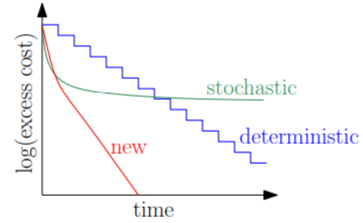
\includegraphics[scale=1]{Image/rates_optim.PNG}
    \caption{The desired convergence \textit{(image taken from \cite{slides})}}
    \label{fig:fig1}
\end{figure}

\section{Variance Reduced Stochastic Gradient Descent}
\subsection{Main idea}

In order to find this new method, we will modify the usual update rule of the SGD. Usually, in the SGD algorithm, we have:

\begin{equation}
    w_{t} = w_{t-1} - \gamma_t \nabla f_{i_t}(w_{t-1})
\end{equation}
with $\gamma_t$ the learning rate and $i_t \in [\![1,n]\!]$ the randomly picked index  at iteration $t$. If we consider the random variables  $i_t \sim \mathcal{U}([\![1,n]\!])$, then the $X^{(t)}(i_t) \eqbydef \nabla f_{i_t}(w_{t-1})$ are also random variables. We then have $\mathbb{E}_{i_t \sim \mathcal{U}}[X^{(t)}] = \frac{1}{n} \sum_i X^{(t)}(i_t=i)$ is the batch gradient in the GD method. We would like to use $\mathbb{E}[X^{(t)}]$ instead of the $X^{(t)}$, the problem being it is expensive to compute. One way to solve that would be to use Monte Carlo samples to estimate $\mathbb{E}[X^{(t)}]$ using random variables $Y^{(t)}$ \textbf{highly correlated} with the $X^{(t)}$ but for which the \textbf{expectation is cheap to compute}. Let's consider the following parametrized estimator of $\mathbb{E}[X^{(t)}]$:
\begin{equation}
    \forall \alpha \in [0,1], \; \theta_{\alpha}^{(t)} \eqbydef \alpha \big(X^{(t)}(i_t)-Y^{(t)}(i_t) \big ) + \mathbb{E}[Y^{(t)}]
\end{equation}

Then, we have the following properties:

\begin{align}
    \mathbb{E}[\theta_{\alpha}^{(t)}] & = \alpha \mathbb{E}[X^{(t)}] +(1-\alpha)\mathbb{E}[Y^{(t)}] \\
    \mathbb{V}[\theta_{\alpha}^{(t)}] & = \alpha^2 \Big[ \mathbb{V}[X^{(t)}] + \mathbb{V}[Y^{(t)}] - 2 Cov(X^{(t)},Y^{(t)}) \Big] 
\end{align}

\begin{itemize}
    \item From (20.4) we deduce that $\theta_{\alpha}^{(t)}$ is \textbf{unbiased} if $\mathbb{E}[X^{(t)}] = \mathbb{E}[Y^{(t)}]$ \textit{(which is not interesting as we wouldn't need sampling)} or if $\alpha = 1$
    \item From (20.5) we deduce that $\theta_{\alpha}^{(t)}$ has \textbf{low variance} if $\alpha$ is small or if $Y^{(t)}$ is highly correlated with $X^{(t)}$
\end{itemize}
Then, in this setting, what remains to be done is \textbf{setting $\alpha$} and \textbf{finding good $Y^{(t)}$} to use $\theta_\alpha^{(t)}$ instead of $X^{(t)}$ in (20.2). In the next subsection, we will present the $3$ different choices made for the variance reduced techniques SAG \textit{(Stochastic Average Gradient)}, SAGA \textit{(Stochastic Average Gradient Amélioré)} and SVRG \textit{(Stochastic Variance Reduced Gradient)}.

\subsection{3 update rules}
Let's introduce $g^{(t)}$ the past stored gradients \textit{(in practice it is a table containing the last gradient computed at each training example)}. If we set an other random variable $i_t^{'} \sim \mathcal{U}([\![1,n]\!])$, we can identify $g^{(t)}(i_t^{'} |i_t)$ as the following r.v:
$$
 g^{(t)}(i_t^{'} |i_t) \eqbydef \left\{
    \begin{array}{ll}
        X^{(t)} = \nabla f_{i_t}(w_{t-1}) & \mbox{if } i_t^{'}=i_t \\
        g^{(t-1)}(i_t^{'}) & \mbox{otherwise}
    \end{array}
\right.
$$
Then, at time step $t$, the only element that changes in $g^{(t)}$ compared to $g^{(t-1)}$ is $g_{i_t}$ which is updated. With this definition we have that $g^{(t)}(i_t) = X^{(t)}$ and $\mathbb{E}_{i_t^{'} \sim \mathcal{U}}[g^{(t)}] = \frac{1}{n} \sum_{i} g^{(t)}(i_t^{'}=i)$.
\begin{itemize}
    \item \textbf{SAG/SAGA} : $Y^{(t)}=g^{(t-1)}$:
    \begin{itemize}
        \item \textbf{SAG}: $\alpha = \frac{1}{n}$. Then, in this setting, combining (20.3) and (20.2) gives:
        \begin{align}
            w_{t} &= w_{t-1} - \gamma_t \Big( \overbrace{\dfrac{1}{n}}^{\alpha} \big[ \overbrace{\nabla f_{i_t}(w_{t-1})}^{X^{(t)}(i_t) = g_{i_t}^{(t)}} - \overbrace{g_{i_t}^{(t-1)}}^{Y^{(t)}(i_t)} \big] + \overbrace{\dfrac{1}{n}\sum_j g_j^{(t-1)}}^{\mathbb{E}[Y^{(t)}]} \Big) \\
            w_{t} &= w_{t-1} - \gamma_t \Big(\dfrac{1}{n}\sum_j g_j^{(t)} \Big)
        \end{align}
        Thus, SAG is \textbf{biased} ($\alpha \neq 1$) but its variance goes to $0$ as $n \rightarrow \infty$ and we have \textbf{low variance}.
        
        \item \textbf{SAGA}: $\alpha = 1$. Then, the update rule is:
        \begin{align}
            w_{t} &= w_{t-1} - \gamma_t \Big( \overbrace{1}^{\alpha} \times \big[\overbrace{\nabla f_{i_t}(w_{t-1})}^{X^{(t)}(i_t) = g_{i_t}^{(t)}} - \overbrace{g_{i_t}^{(t-1)}}^{Y^{(t)}(i_t)} \big] + \overbrace{\dfrac{1}{n}\sum_j g_j^{(t-1)}}^{\mathbb{E}[Y^{(t)}]} \Big) \\
            w_{t} &= w_{t-1} - \gamma_t \Big(g_{i_t}^{(t)} - g_{i_t}^{(t-1)} + \dfrac{1}{n}\sum_j g_j^{(t-1)} \Big)
        \end{align}
        Here, we see that SAGA is \textbf{unbiased} ($\alpha=1$), but then the variance is $n^2$ higher than in SAG. The "variance reduction" only comes from the correlation between $X^{(t)}$ and $Y^{(t)}$
    \end{itemize}
    
    \item \textbf{SVRG}: Here, we pose $\alpha = 1$ and $Y^{(t)}(i_t) = \nabla f_{i_t}(w_{old})$. The idea is to compute the $n$ gradients every few steps and use them without updating them during $T_{max}$ steps. This procedure then allows us to store in memory only $g_{ref} = \mathbb{E}[Y^{(t)}]$ and $w_{old}$ \textit{(which is significantly less than a table of $n$ gradients)} at the cost of computing at least $2$ derivatives at each iteration ($\nabla f_{i_t}(w_{t-1})$ and $\nabla f_{i_t}(w_{old})$ ).
    \begin{align}
            w_{t} &= w_{t-1} - \gamma_t \Big(\nabla f_{i_t}(w_{t-1}) - \nabla f_{i_t}(w_{old}) + \underbrace{\dfrac{1}{n}\sum_j \nabla f_{j}(w_{old})}_{g_{ref}} \Big)
    \end{align}
    Then, the method is \textbf{unbiased} and the \textbf{memory footprint of SVRG is much lower} than for SAG/SAGA. But the computation is a bit heavier in average at each step and the user has to tune $T_{max}$. In the next subsection, we will discuss a bit the properties of those methods.
\end{itemize}

\begin{paragraph}
{Note: } \textit{SAG/SAGA can easily be used for generalized linear models where the dependence of the $f_i$ on the $x_i$ is of the form $<w, x_i>$, allowing the table of gradients to only store scalars. But for more complex loss function it may not be suitable (e.g for deep neural networks).}
\end{paragraph}

\subsection{Properties}

\begin{algorithm}[H]
\SetAlgoLined
\KwResult{$w^{(m)}$}
 initialization of $w^{(0)}$\;
 \For{$k=0,...,m$}{
  $g_{ref} \eqbydef \frac{1}{n} \sum_j \nabla f_j(w^{(k)})$\;
  
  \For{$t=0,..., T_{max}$}{
   sample $i_t \sim \mathcal{U}([\![1,n]\!])$\;
   $w_{t}^{(k)} = w_{t-1}^{(k)} - \gamma_t \Big(\nabla f_{i_t}(w_{t-1}^{(k)}) - \nabla f_{i_t}(w^{(k)}) + g_{ref} \Big)$;
   }{
   $w^{(k+1)} = w_{T_{max}}^{(k)}$;
  }
 }
 \caption{SVRG algorithm}
\end{algorithm}

From the SVRG algorithm, two questions main questions arise:\textit{ What should be $\gamma_t$ ?} and \textit{ What should be $T_{max}$ ?}
\\
\\
The original SVRG convergence results give:
\begin{itemize}
    \item $\gamma_t \leq \dfrac{1}{L}$ with $L$ the Lipschitz constant
    \item $T_{max} \geq \dfrac{L}{\mu} = \kappa$ with $\kappa$ the condition number
\end{itemize}
Then, as $\kappa$ is needed, the method is not adaptive to local strong convexity: there is a need to know the strong convexity properties of the loss before running the method, which is more than the SAG/SAGA methods demand \textit{(they are adaptive)}. But with a tweak on SVRG, better properties fall \cite{Hofmann2015}:
\\
\\
If $T_{max} \sim Geom(\frac{1}{n})$ \textit{(i.e at each inner loop iteration the inner loop is ended with probability $\frac{1}{n}$)}, then the same convergence properties as SAGA fall. Moreover, we have $\mathbb{E}[T_{max}] = n$ and the overall cost of SVRG $\simeq 3 \times$ (SGD for each $n$ updates).
\\
With this tweak, then for the three algorithms SAG/SAGA/SVRG the rate of convergence for convex functions ($\mu = 0$) get $\min_t \big[ \mathbb{E} f(w_t) - f^* \big] = O(1/t)$ which contrast with the $O(1/\sqrt{t})$ rate for the SGD.

\begin{figure}[h]
    \centering
    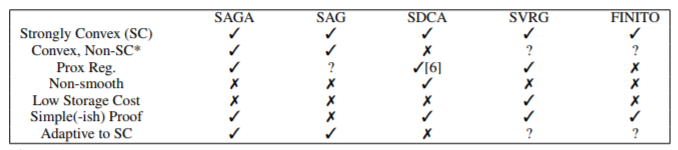
\includegraphics[scale=1]{Image/summary.PNG}
    \caption{Summary of a few variance reduced optimization methods \textit{(image taken from \cite{DefazioBL14}). This photo is older than the results in \cite{Hofmann2015}}}
    \label{fig:fig2}
\end{figure}

\section{Application to CRF}

\section{Proximal gradient method}
%----------------------------------------
\bibliographystyle{plain}
\bibliography{notes}
%----------------------------------------
\end{document}
%%% Local Variables:
%%% mode: latex
%%% TeX-master: t
%%% End:
